\chapter{麦克斯韦方程组、协变性与电磁波}

\lectureoverview{电场和磁场通过洛伦兹力作用于带电物质，但物质也必须产生并重新排布场。我们将表述电磁学的这另一半互易关系，证明麦克斯韦方程组是洛伦兹协变的，导出其波动解，然后以使局域守恒显而易见的形式重新引入电荷和电流。在整个讲座中，我们使用\(c=1\)的单位制。}

\section{电磁学的另一半}

从已经掌握的那部分内容开始。若一个电荷为\(q\)的粒子以速度\(\mathbf v\)穿过电场和磁场，则力为
\begin{equation}
\mathbf F=q\bigl(\mathbf E+\mathbf v\times\mathbf B\bigr).
\label{eq:lorentz-force-three}
\end{equation}
因子\(q\)不可或缺。不带电的粒子感受不到电磁力。即使粒子瞬时静止，电场也有贡献，而磁场的贡献则取决于其运动。

方程~\eqref{eq:lorentz-force-three}告诉我们给定的场对物质做了什么。它并未告诉我们是什么决定了场。是什么在一个物体周围产生电场、在另一个物体周围产生磁场，或产生一个在真空中传播的波？回答这些问题的方程就是麦克斯韦方程组。

\begin{figure}[H]
\centering
\includegraphics[width=0.62\textwidth]{lecture_58_figure_02.png}
\caption{三矢量洛伦兹力及其张量重述的开端。}
\lectureframe{00:05:49}
\end{figure}

力定律的相对论形式预示了我们所需的记号：
\begin{equation}
f^\mu=qF^\mu{}_{\nu}u^\nu.
\label{eq:lorentz-force-four}
\end{equation}
这里\(u^\nu\)是四维速度，\(f^\mu\)是四维力，而\(F^{\mu\nu}\)是由\(\mathbf E\)和\(\mathbf B\)组装成的反对称张量。黑板上首先只显示了这个表达式的示意性开端；与\(u^\nu\)的缩并提供了留下一个自由力指标所需的缺失矢量。

物质必须反作用于场，这有一个物理上的理由。电磁波可以击中一个电荷，使其加速，并把能量传递给它。如果场能影响电荷，而电荷却永远不能影响场，那么这份能量就没有来源可供抽取。作用与反作用并不完全是全部论证，但能量守恒使这种互易耦合不可避免。

\section{变化的源发出扰动}

一个点电荷产生一个从其位置向外或向内指向的电场。导线中的电流--带电粒子的流动--产生一个环绕导线环流的磁场。这些熟悉的静态图像已经显示出两种不同的几何模式：电通量从电荷发出，而磁感线则绕电流缠绕。

现在突然移动这个点电荷。在其新位置附近，电场必须开始重新排布，但远处的观察者无法立即得知这一运动。在信号有时间到达之前，旧的场仍留在远处。在近区和远区之间，存在一个场正在变化的移动前沿。这种移动的重新排布就是一种电磁扰动。

如果电荷被来回驱动，相继的重新排布便一个接一个地发生，形成电磁波。这就是天线的基本功能：振荡的电流向外发出场的扰动。使导线中的电流反向，就给出同一论证的磁版本。\(\mathbf B\)的环流必须反向，但这一反向是传播的，而不是同时出现在各处。

这一因果图像为麦克斯韦方程组设定了两个目标。它们必须描述电荷和电流如何作为场的源，并且必须允许这些场的变化以不快于光速的速度传播。第二个目标也是对相对论的检验。如果麦克斯韦方程组在每个惯性系中都有相同的形式，并蕴含一个确定的波速，那么每个惯性系都必定由它们推断出相同的速度。

\section{回顾相对论波动方程}

在转向矢量场之前，先考虑一个标量场\(\phi(\mathbf x,t)\)，即在每个时空点处有一个数。一个一阶导数方程
\begin{equation}
\partial_\mu\phi=0
\end{equation}
将意味着每个时空导数都为零。该场将是常量，因而无法承载波。一个非平凡的相对论波动方程使用两个导数：
\begin{equation}
\partial_\mu\partial^\mu\phi=0.
\end{equation}
按照这里使用的符号约定，
\begin{equation}
\left(\partial_t^2-\partial_x^2-\partial_y^2-\partial_z^2\right)\phi=0,
\label{eq:scalar-wave-four}
\end{equation}
或者更紧凑地，
\begin{equation}
\left(\partial_t^2-\nabla^2\right)\phi=0.
\end{equation}
选择\(c=1\)使时间和距离具有相容的单位。恢复普通单位会把\(1/c^2\)放在二阶时间导数旁边。

对于沿\(z\)轴传播的波，场依赖于\(z\)和\(t\)，而不依赖于\(x\)或\(y\)。方程~\eqref{eq:scalar-wave-four}简化为
\begin{equation}
\left(\partial_t^2-\partial_z^2\right)\phi=0.
\label{eq:scalar-wave-one}
\end{equation}

\begin{figure}[H]
\centering
\includegraphics[width=0.56\textwidth]{lecture_58_figure_04.png}
\caption{用作电磁波模型的一维标量波动方程。}
\lectureframe{00:47:03}
\end{figure}

它的一般行波形式为
\begin{equation}
\phi(z,t)=f(z-t)+g(z+t).
\end{equation}
剖面\(f(z-t)\)朝\(z\)增大的方向移动，因为相位固定的点满足\(z-t=\text{constant}\)。剖面\(g(z+t)\)朝相反方向移动。没有任何条件要求这两个剖面中的任何一个必须是正弦式的；任何足够光滑的形状都会在不改变形式的情况下平移。

不过正弦波用起来很方便：
\begin{equation}
\phi(z,t)=A\cos\!\bigl(k(z-t)\bigr).
\end{equation}
波数\(k\)控制波长，
\begin{equation}
\lambda=\frac{2\pi}{k}.
\end{equation}
大的\(k\)产生快速的空间振荡和短的波长；小的\(k\)产生长的波长。这些同样的剖面很快就会成为\(\mathbf E\)和\(\mathbf B\)的分量。

\section{麦克斯韦方程组所需的向量微积分}

麦克斯韦方程组是用点积、叉积、散度和旋度写出的。值得把记号重新建立一次，因为后面的分量计算恰恰要用到这些模式。

对于普通的三维向量\(\mathbf a\)和\(\mathbf b\)，点积是标量
\begin{equation}
\mathbf a\cdot\mathbf b
=a_xb_x+a_yb_y+a_zb_z.
\end{equation}
叉积是另一个向量，
\begin{align}
(\mathbf a\times\mathbf b)_x&=a_yb_z-a_zb_y,\\
(\mathbf a\times\mathbf b)_y&=a_zb_x-a_xb_z,\\
(\mathbf a\times\mathbf b)_z&=a_xb_y-a_yb_x.
\end{align}
其余分量由循环次序\(x\to y\to z\to x\)得出。

引入微分算子
\begin{equation}
\boldsymbol\nabla=
\left(\partial_x,\partial_y,\partial_z\right).
\end{equation}
它的各个元素是算子而不是普通数，但点积和叉积的模式仍然可以使用。对于向量场\(\mathbf A\)，
\begin{equation}
\boldsymbol\nabla\cdot\mathbf A
=\partial_xA_x+\partial_yA_y+\partial_zA_z
\label{eq:divergence}
\end{equation}
是散度，而
\begin{align}
(\boldsymbol\nabla\times\mathbf A)_x
 &=\partial_yA_z-\partial_zA_y,\\
(\boldsymbol\nabla\times\mathbf A)_y
 &=\partial_zA_x-\partial_xA_z,\\
(\boldsymbol\nabla\times\mathbf A)_z
 &=\partial_xA_y-\partial_yA_x
\label{eq:curl}
\end{align}
是旋度的各个分量。

几何图像与公式同样重要。向量场在看起来从源向外流出的地方具有正的散度。它在发生环流的地方具有旋度。点电荷的径向电场说明了散度；环绕载流导线的磁场说明了旋度。空间上恒定的向量场两者都没有。

\section{真空中的麦克斯韦方程组}

在没有电荷和电流的情况下，麦克斯韦方程组为
\begin{align}
\boldsymbol\nabla\times\mathbf E&=-\partial_t\mathbf B,
\label{eq:faraday-vac}\\
\boldsymbol\nabla\cdot\mathbf B&=0,
\label{eq:gauss-b-vac}\\
\boldsymbol\nabla\times\mathbf B&=\partial_t\mathbf E,
\label{eq:ampere-vac}\\
\boldsymbol\nabla\cdot\mathbf E&=0.
\label{eq:gauss-e-vac}
\end{align}
两个旋度方程几乎交换了\(\mathbf E\)和\(\mathbf B\)，但一个关键的负号把它们区分开来。两个散度方程说明，在所考虑的真空区域内，两个场都没有源。即使恢复电的源，磁的散度仍然为零；普通电磁学中不包含磁荷。

\begin{figure}[H]
\centering
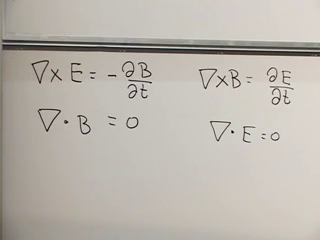
\includegraphics[width=0.76\textwidth]{lecture_58_figure_06.png}
\caption{四个真空麦克斯韦方程，其排列方式显示出电场与磁场之间的近似对称性。}
\lectureframe{00:27:30}
\end{figure}

电荷密度\(\rho\)最终将取代方程~\eqref{eq:gauss-e-vac}右端的零，电流密度\(\mathbf J\)将进入方程~\eqref{eq:ampere-vac}。我们暂时推迟这些项。无源方程以最少的杂乱揭示了变换结构和波动机制。

它们也使爱因斯坦的难题更加尖锐。一个跟随波运动的伽利略观察者会期望减去速度并测得较小的波速。然而，如果同样的麦克斯韦方程组在每个惯性系中都成立，那么每个观察者都会导出相同的单位波速。出路不是在不同参考系之间改变波动方程。而是使用洛伦兹变换，并把麦克斯韦方程组用变换规律已知的对象表示出来。

\section{电场与磁场作为一个张量}

电场和磁场组合成反对称场张量
\begin{equation}
F^{\mu\nu}=
\begin{pmatrix}
0   & -E_x & -E_y & -E_z\\
E_x & 0    & -B_z & B_y\\
E_y & B_z  & 0    & -B_x\\
E_z & -B_y & B_x  & 0
\end{pmatrix},
\label{eq:l0203-field-tensor}
\end{equation}
其中行和列的次序为\(t,x,y,z\)。反对称性，
\begin{equation}
F^{\mu\nu}=-F^{\nu\mu},
\end{equation}
迫使对角元为零，并由上半部分确定矩阵的下半部分。时间-空间元包含\(\mathbf E\)；纯空间元包含\(\mathbf B\)。

\begin{figure}[H]
\centering
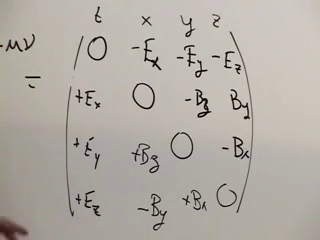
\includegraphics[width=0.58\textwidth]{lecture_58_figure_03.png}
\caption{完整的电磁场张量，包括其电的和磁的元。}
\lectureframe{00:32:05}
\end{figure}

\(F^{\mu\nu}\)的重要性不仅仅在于六个场分量能装进一个矩阵。在洛伦兹变换下，它作为二阶张量变换。因此，不同观察者测得的电场和磁场恰好以整个对象协调变换所需的方式混合。

还有第二个反对称张量，即对偶场张量\(\widetilde F^{\mu\nu}\)。在目前的约定下，它由方程~\eqref{eq:l0203-field-tensor}通过替换
\begin{equation}
\mathbf E\longmapsto-\mathbf B,
\qquad
\mathbf B\longmapsto\mathbf E.
\label{eq:dual-replacement}
\end{equation}
得到。因此
\begin{equation}
\widetilde F^{\mu\nu}=
\begin{pmatrix}
0    & B_x  & B_y  & B_z\\
-B_x & 0    & -E_z & E_y\\
-B_y & E_z  & 0    & -E_x\\
-B_z & -E_y & E_x  & 0
\end{pmatrix}.
\label{eq:dual-tensor}
\end{equation}
方程~\eqref{eq:dual-replacement}中的符号很重要。讲座先口头尝试交换，发现符号不匹配，并在完成矩阵之前加以修正。

\begin{figure}[H]
\centering
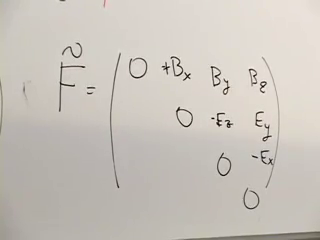
\includegraphics[width=0.58\textwidth]{lecture_58_figure_07.png}
\caption{通过以所需的符号交换电的和磁的元来组装对偶张量。}
\lectureframe{00:35:45}
\end{figure}

\section{协变的真空方程}

每个麦克斯韦方程都包含一个导数。从一个二阶张量出发并缩并一个导数指标后，剩下一个自由指标，因此自然的协变候选是
\begin{align}
\partial_\mu F^{\mu\nu}&=0,
\label{eq:maxwell-covariant-vac}\\
\partial_\mu\widetilde F^{\mu\nu}&=0.
\label{eq:maxwell-dual-vac}
\end{align}
对于\(\nu\)的每个固定值，方程~\eqref{eq:maxwell-covariant-vac}是一个方程。由于\(\nu\)可以是\(t,x,y,z\)，它打包了四个标量方程。方程~\eqref{eq:maxwell-dual-vac}打包了另外四个。这与原始列表中的两个矢量旋度方程和两个标量散度方程相符。

紧凑记号只有在能重现熟悉的方程时才有用。取\(\nu=z\)：
\begin{align}
\partial_\mu F^{\mu z}
&=\partial_tF^{tz}
  +\partial_xF^{xz}
  +\partial_yF^{yz}
  +\partial_zF^{zz}\\
&=-\partial_tE_z+\partial_xB_y-\partial_yB_x\\
&=-\partial_tE_z+
  \bigl(\boldsymbol\nabla\times\mathbf B\bigr)_z.
\end{align}
项\(F^{zz}\)因反对称性而消失。令结果为零，得到
\begin{equation}
\boldsymbol\nabla\times\mathbf B=\partial_t\mathbf E.
\end{equation}
的\(z\)分量。通过循环指标可得\(x\)和\(y\)分量。

\begin{figure}[H]
\centering
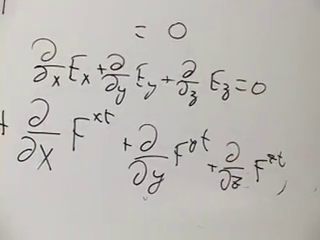
\includegraphics[width=0.76\textwidth]{lecture_58_figure_08.png}
\caption{协变场方程的分量展开；对角张量分量消失，其余项重构出麦克斯韦方程组。}
\lectureframe{00:43:30}
\end{figure}

现在取时间分量：
\begin{align}
\partial_\mu F^{\mu t}
&=\partial_tF^{tt}
  +\partial_xF^{xt}
  +\partial_yF^{yt}
  +\partial_zF^{zt}\\
&=\partial_xE_x+\partial_yE_y+\partial_zE_z\\
&=\boldsymbol\nabla\cdot\mathbf E.
\end{align}
因此它给出方程~\eqref{eq:gauss-e-vac}。对偶张量进行同样的检验得到
\(\boldsymbol\nabla\cdot\mathbf B=0\)和
\(\boldsymbol\nabla\times\mathbf E=-\partial_t\mathbf B\)。

这些紧凑方程现在已被确立，而不仅仅是猜测。它们的自由指标结构使它们成为四维矢量方程，因此洛伦兹变换改变其分量但不改变其形式。这正是真空麦克斯韦方程在每个惯性系中都相同的精确含义。

\section{从一阶方程到波}

麦克斯韦方程只包含一阶导数，而波动方程包含二阶导数。这一表面上的不匹配之所以得到解决，是因为麦克斯韦理论耦合了两个场。关于\(\mathbf E\)和\(\mathbf B\)的一对方程可以合并为关于任一单独场的二阶方程。

将方程~\eqref{eq:ampere-vac}对时间求导：
\begin{equation}
\partial_t^2\mathbf E
=\boldsymbol\nabla\times\partial_t\mathbf B.
\end{equation}
法拉第定律给出\(\mathbf B\)的时间导数，
\begin{equation}
\partial_t\mathbf B=-\boldsymbol\nabla\times\mathbf E,
\end{equation}
因此
\begin{equation}
\partial_t^2\mathbf E
=-\boldsymbol\nabla\times
  \bigl(\boldsymbol\nabla\times\mathbf E\bigr).
\label{eq:double-curl}
\end{equation}

黑板上的推导逐分量进行，而不是引用一个记忆中的恒等式。对于\(x\)分量，
\begin{align}
\bigl[\boldsymbol\nabla\times
(\boldsymbol\nabla\times\mathbf E)\bigr]_x
&=\partial_y(\boldsymbol\nabla\times\mathbf E)_z
 -\partial_z(\boldsymbol\nabla\times\mathbf E)_y\\
&=\partial_y(\partial_xE_y-\partial_yE_x)\\
&\quad-\partial_z(\partial_zE_x-\partial_xE_z)\\
&=\partial_x(\partial_yE_y+\partial_zE_z)
 -\partial_y^2E_x\\
&\quad-\partial_z^2E_x.
\end{align}
加减\(\partial_x^2E_x\)以显露出散度：
\begin{align}
\bigl[\boldsymbol\nabla\times
(\boldsymbol\nabla\times\mathbf E)\bigr]_x
&=\partial_x(\boldsymbol\nabla\cdot\mathbf E)
 -\nabla^2E_x.
\label{eq:double-curl-x}
\end{align}
在真空中\(\boldsymbol\nabla\cdot\mathbf E=0\)。结合方程~\eqref{eq:double-curl}和\eqref{eq:double-curl-x}得到
\begin{equation}
\left(\partial_t^2-\nabla^2\right)E_x=0.
\label{eq:ex-wave}
\end{equation}

\begin{figure}[H]
\centering
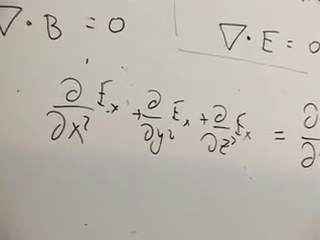
\includegraphics[width=0.72\textwidth]{lecture_58_figure_09.png}
\caption{分量计算得到\(E_x\)的波动方程。}
\lectureframe{00:57:10}
\end{figure}

同样的计算适用于\(E_y\)和\(E_z\)，类似的消元给出
\begin{equation}
\left(\partial_t^2-\nabla^2\right)\mathbf B=0.
\end{equation}
因此电场和磁场可以作为波在真空中传播。在此处使用的单位中，它们的速度为一，这意味着当恢复普通单位时速度为\(c\)。

\section{平面波及其偏振}

构造一个沿\(z\)正方向传播的简单波：
\begin{equation}
\mathbf E(z,t)
=\widehat{\mathbf x}\,E_0
  \cos\!\bigl(k(z-t)\bigr).
\label{eq:plane-e}
\end{equation}
其波形沿\(z\)平移而不改变形状。由于电场沿\(x\)轴指向，该波在\(x\)方向上为线偏振。我们选择\(E_y=0\)只是为了保持例子简单；本可以包含第二个横向偏振。

纵向分量并非同样自由。由于波只依赖于\(z\)和\(t\)，
\begin{equation}
\boldsymbol\nabla\cdot\mathbf E
=\partial_zE_z=0.
\end{equation}
因此\(E_z\)可以是常数，但不能包含变化的波形。均匀背景场可以独立地叠加或移除；它不是传播辐射的一部分。波本身是横波：
\begin{equation}
\mathbf E_{\mathrm{wave}}\cdot\widehat{\mathbf z}=0.
\end{equation}

法拉第定律确定磁场。对于方程~\eqref{eq:plane-e}，\(\boldsymbol\nabla\times\mathbf E\)的唯一非零分量是\(y\)分量，
\begin{equation}
(\boldsymbol\nabla\times\mathbf E)_y=\partial_zE_x.
\end{equation}
因此\(\partial_t\mathbf B\)沿\(y\)指向，一个相容的选择是
\begin{equation}
\mathbf B(z,t)
=\widehat{\mathbf y}\,E_0
  \cos\!\bigl(k(z-t)\bigr).
\label{eq:plane-b}
\end{equation}
在这些单位中，电场和磁场的振幅相等。它们的取向满足
\begin{equation}
\mathbf E\perp\mathbf B,
\qquad
\mathbf E\perp\widehat{\mathbf z},
\qquad
\mathbf B\perp\widehat{\mathbf z},
\qquad
\mathbf E\times\mathbf B\parallel\widehat{\mathbf z}.
\end{equation}

\begin{figure}[H]
\centering
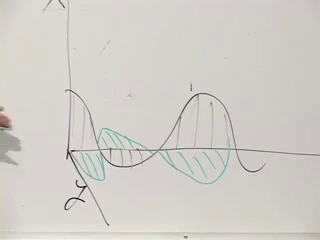
\includegraphics[width=0.70\textwidth]{lecture_58_figure_05.png}
\caption{横电磁波的完整黑板示意图：电场和磁场的振荡彼此垂直，且都垂直于传播方向。}
\lectureframe{01:05:25}
\end{figure}

\begin{figure}[H]
\centering
\scalebox{0.90}{%
\begin{tikzpicture}[x=1cm,y=1cm,>=Latex]
  \draw[->,thick] (0,0) -- (8.2,0) node[right] {$z$};
  \draw[->,thick] (0,-1.6) -- (0,1.7) node[above] {$x$};
  \draw[->,thick] (0,0) -- (-1.15,-0.8) node[below left] {$y$};
  \draw[blue!70!black,thick,domain=0:7.5,samples=120]
    plot (\x,{0.95*sin(90*\x)});
  \foreach \z/\s in {0.8/1,2.8/-1,4.8/1,6.8/-1}{
    \draw[->,green!45!black,thick]
      (\z,0) -- ++({-0.55*\s},{-0.38*\s});
  }
  \node[blue!70!black] at (6.9,1.25) {$\mathbf E$};
  \node[green!45!black] at (5.2,-1.05) {$\mathbf B$};
  \draw[->,very thick] (6.2,1.55) -- (7.7,1.55)
    node[midway,above] {propagation};
\end{tikzpicture}
}
\caption{场\(\mathbf E\)和\(\mathbf B\)彼此垂直，且都垂直于传播方向。}
\end{figure}

这就是光以及真空中所有电磁辐射的特征。由于产生该波的方程是洛伦兹协变的，另一个惯性观察者同样会描述一个以\(c\)运动的电磁波，具有横向的电场和磁场。

\section{电荷密度与电流密度}

现在恢复此前暂时搁置的源。当许多带电粒子占据一个区域时，将它们粗粒化为连续电荷密度是方便的
\begin{equation}
\rho(\mathbf x,t)=\frac{dQ}{dV}.
\end{equation}
这种近似就像把水当作连续流体来处理，尽管水由分子组成。正电荷与负电荷以相反的符号贡献，因此\(\rho\)是单位体积的净电荷。

所选区域\(V\)内的电荷为
\begin{equation}
Q_V(t)=\int_V\rho(\mathbf x,t)\,dV.
\label{eq:charge-volume}
\end{equation}
密度可以随位置和时间变化。一堆电荷可以从某点移走，从而改变该处的局域密度。然而，它不能以任意方式变化。自然界守恒电荷。

仅全局守恒太弱。它会允许电荷在同一瞬间从地球消失并在火星出现，而总量保持不变。更强的陈述是局域的：电荷只能通过中间空间中的流动离开一处并到达另一处。

为了描述这种流动，取一个无穷小有向面元
\begin{equation}
d\boldsymbol\sigma=\widehat{\mathbf n}\,d\sigma.
\end{equation}
其大小是面积，其方向垂直于表面。电流密度\(\mathbf J\)的定义使得单位时间穿过该面元的电荷为
\begin{equation}
\frac{dQ}{dt}=\mathbf J\cdot d\boldsymbol\sigma.
\label{eq:current-flux-element}
\end{equation}
\(\mathbf J\)的大小是单位面积单位时间的电荷，其方向是正电荷流动的方向。

\begin{figure}[H]
\centering
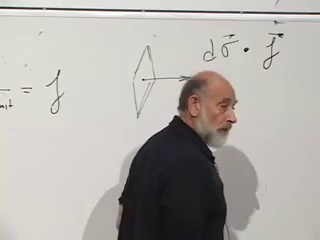
\includegraphics[width=0.64\textwidth]{lecture_58_figure_10.png}
\caption{有向面元与通量因子\(d\boldsymbol\sigma\cdot\mathbf J\)。}
\lectureframe{01:18:15}
\end{figure}

点积选出垂直于表面的分量。与表面相切的电流不穿过任何一侧，贡献为零。平行于法线的电流在大小固定时给出最大通量。导线电流是一种特殊情况，但\(\mathbf J\)也可以描述穿过薄片或在整个三维空间中流动的电荷。

\section{局域守恒与连续性方程}

固定空间中的一个区域\(V\)，并将其闭合边界\(\partial V\)的每个面元取为外法向。如果存在净向外的电流，则内部电荷减少：
\begin{equation}
\frac{dQ_V}{dt}
=-\oint_{\partial V}\mathbf J\cdot d\boldsymbol\sigma.
\label{eq:integral-conservation}
\end{equation}
负号是物理的而非约定的：正的向外通量从该区域移走正电荷。利用方程~\eqref{eq:charge-volume}，
\begin{equation}
\int_V\partial_t\rho\,dV
=-\oint_{\partial V}\mathbf J\cdot d\boldsymbol\sigma.
\label{eq:integral-continuity-one}
\end{equation}

\begin{figure}[H]
\centering
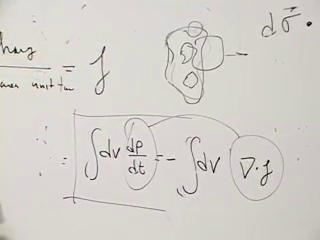
\includegraphics[width=0.72\textwidth]{lecture_58_figure_11.png}
\caption{将表面通量转化为体积陈述后的固定区域守恒定律。}
\lectureframe{01:29:00}
\end{figure}

高斯定理，也称为散度定理，将穿过闭合曲面的通量与其内部的散度联系起来：
\begin{equation}
\oint_{\partial V}\mathbf A\cdot d\boldsymbol\sigma
=\int_V\boldsymbol\nabla\cdot\mathbf A\,dV.
\label{eq:divergence-theorem}
\end{equation}
可以想象隐藏的管道在容器内部的各点注入水。散度衡量水从管端冒出的局域速率；面积分衡量离开容器的总水量。内部作为向外流动而被创造出来的东西，最终必须穿过边界。

将方程~\eqref{eq:divergence-theorem}应用于\(\mathbf J\)得到
\begin{equation}
\int_V
\left(\partial_t\rho+\boldsymbol\nabla\cdot\mathbf J\right)dV=0.
\end{equation}
此关系对每一个可能的区域\(V\)都成立。因此被积函数必须逐点为零：
\begin{equation}
\boxed{\partial_t\rho+\boldsymbol\nabla\cdot\mathbf J=0.}
\label{eq:continuity-three}
\end{equation}

\begin{figure}[H]
\centering
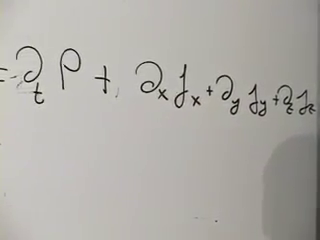
\includegraphics[width=0.72\textwidth]{lecture_58_figure_12.png}
\caption{逐分量写出的局域连续性方程。}
\lectureframe{01:29:50}
\end{figure}

方程~\eqref{eq:continuity-three}恰好说明了局域守恒所要求的内容。如果电荷密度在某点或小区域内减少，电流必须从该处向外发散。如果电流向内汇聚，电荷密度就增加。

密度和电流自然地组成四维电流
\begin{equation}
J^\mu=(\rho,J_x,J_y,J_z)
\label{eq:four-current}
\end{equation}
在\(c=1\)单位下。连续性方程变为洛伦兹标量方程
\begin{equation}
\partial_\mu J^\mu=0.
\label{eq:continuity-four}
\end{equation}
相对论性分布的流动应当像单个粒子的四维速度一样按四维矢量变换。方程~\eqref{eq:continuity-four}使局域电荷守恒在每个惯性系中都成立。

\section{有源的麦克斯韦方程组}

恢复电荷和电流后得到
\begin{align}
\boldsymbol\nabla\cdot\mathbf E&=\rho,
\label{eq:gauss-e-source}\\
\boldsymbol\nabla\cdot\mathbf B&=0,\\
\boldsymbol\nabla\times\mathbf E&=-\partial_t\mathbf B,\\
\boldsymbol\nabla\times\mathbf B&=\partial_t\mathbf E+\mathbf J.
\label{eq:ampere-source}
\end{align}
涉及电性源的方程合并为
\begin{equation}
\boxed{\partial_\mu F^{\mu\nu}=J^\nu,}
\label{eq:maxwell-source-covariant}
\end{equation}
而无源的磁方程对仍为
\begin{equation}
\boxed{\partial_\mu\widetilde F^{\mu\nu}=0.}
\label{eq:maxwell-dual-source}
\end{equation}

\begin{figure}[H]
\centering
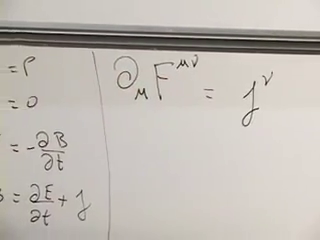
\includegraphics[width=0.78\textwidth]{lecture_58_figure_13.png}
\caption{有源麦克斯韦方程组及其协变形式\(\partial_\mu F^{\mu\nu}=J^\nu\)。}
\lectureframe{01:34:00}
\end{figure}

方程~\eqref{eq:maxwell-source-covariant}的时间分量读作
\begin{equation}
\partial_\mu F^{\mu t}=J^t=\rho,
\end{equation}
而已经完成的分量计算将其左侧化为
\(\boldsymbol\nabla\cdot\mathbf E\)。三个空间分量重现
\(\boldsymbol\nabla\times\mathbf B=\partial_t\mathbf E+\mathbf J\)。

还有一个有用的一致性检验。将\(\partial_\nu\)作用于
方程~\eqref{eq:maxwell-source-covariant}得到
\begin{equation}
\partial_\nu J^\nu
=\partial_\nu\partial_\mu F^{\mu\nu}=0,
\end{equation}
因为两个导数在\(\mu\leftrightarrow\nu\)下对称，而\(F^{\mu\nu}\)是反对称的。\editorialnote{这个简短的一致性检验由协变方程得出，并明确说明了为什么有源麦克斯韦方程组自动满足连续性方程。}

互反结构至此完备。张量力定律
\(f^\mu=qF^\mu{}_\nu u^\nu\)描述了场如何作用于电荷，而
方程~\eqref{eq:maxwell-source-covariant}描述了电荷与电流如何产生场。二者均为张量方程。在真空中，同一组场方程给出以\(c\)传播的横波。因此，洛伦兹协变性与电磁波方程在当初促使这一构造的关节点上汇合：每个惯性观测者都得到相同的电磁学定律和相同的光速。